%% LyX 2.3.0 created this file.  For more info, see http://www.lyx.org/.
%% Do not edit unless you really know what you are doing.
\documentclass[english]{beamer}
\usepackage{lmodern}
\renewcommand{\sfdefault}{lmss}
\renewcommand{\ttdefault}{lmtt}
\usepackage[T1]{fontenc}
\usepackage[latin9]{inputenc}
\usepackage{amsmath}
\usepackage{amssymb}
\usepackage{graphicx}
\usepackage{wasysym}
\usepackage{xargs}[2008/03/08]
\usepackage[all]{xy}

\makeatletter

%%%%%%%%%%%%%%%%%%%%%%%%%%%%%% LyX specific LaTeX commands.
%% Because html converters don't know tabularnewline
\providecommand{\tabularnewline}{\\}

%%%%%%%%%%%%%%%%%%%%%%%%%%%%%% Textclass specific LaTeX commands.
% this default might be overridden by plain title style
\newcommand\makebeamertitle{\frame{\maketitle}}%
% (ERT) argument for the TOC
\AtBeginDocument{%
  \let\origtableofcontents=\tableofcontents
  \def\tableofcontents{\@ifnextchar[{\origtableofcontents}{\gobbletableofcontents}}
  \def\gobbletableofcontents#1{\origtableofcontents}
}

%%%%%%%%%%%%%%%%%%%%%%%%%%%%%% User specified LaTeX commands.
\usetheme{Warsaw}
\usepackage{svg}
% or ...

\setbeamercovered{transparent}
% or whatever (possibly just delete it)
\usepackage{etoolbox}
\setbeamertemplate{headline}{%
\leavevmode%
  \hbox{%
    \begin{beamercolorbox}[wd=\paperwidth,ht=2.5ex,dp=1.125ex]{palette quaternary}%
    \insertsectionnavigationhorizontal{\paperwidth}{}{\hskip0pt plus1filll}
    \end{beamercolorbox}%
  }
}
\addtobeamertemplate{navigation symbols}{}{%
    \usebeamerfont{footline}%
    \usebeamercolor[fg]{footline}%
    \hspace{1em}%
    \insertframenumber/\inserttotalframenumber
}
\usepackage{tikz}
\usetikzlibrary{shapes,arrows,positioning}
\usetikzlibrary{decorations.pathreplacing,tikzmark,calc}

\tikzstyle{triangle}=[fill=blue!20, regular polygon, regular polygon sides=3]

%\newcommand{\tikzmark}[1]{\tikz[overlay,remember picture] \node[baseline] (#1) {};}

\tikzset{My Node Style/.style={midway, right, xshift=3.0ex, 
%align=left,
%anchor=west, 
%anchor=north west,
font=\small, draw=none, 
% align=left,
anchor=base west,
 thin, text=black}}

\newcommand\VerticalBrace[4][]{%
    % #1 = draw options
    % #2 = top mark
    % #2 = bottom mark
    % #4 = label
\begin{tikzpicture}[overlay,remember picture]
\path let \p1=(pic cs:#2),\p2=(pic cs:#3) in coordinate (Q1) at ({max(\x1,\x2)+.5em},\y1);
  \draw[decorate,decoration={brace, amplitude=1.5ex}, #1] 
%    ([yshift=1ex]:#2.north east)  --  (#3.south east-|#2.north east)
    ([yshift=1ex]{{pic cs:#2}-|Q1})  --  ({pic cs:#3} -| Q1)
        node[My Node Style
%, baseline=brace.east
] {#4};
\end{tikzpicture}
}
\newcommand{\xyR}[1]{%
\xydef@\xymatrixrowsep@{#1}
} % end of \xyR
\setbeamertemplate{navigation symbols}{%
    \usebeamerfont{footline}%
    \usebeamercolor[fg]{footline}%
    \hspace{1em}%
    \insertframenumber/\inserttotalframenumber
}
\definecolor{green}{RGB}{0,100,0}

\setbeamercolor{alerted text}{fg=blue}

\makeatother

\usepackage{babel}
\usepackage[bibstyle=authoryear,citestyle=verbose]{biblatex}
\begin{document}

\title[Signatures and models for syntax and operational semantics]{Signatures and models for syntax and operational semantics in the
presence of variable binding}

\author{Ambroise Lafont\inst{1}}

\institute[IMT]{\inst{1}DAPI\\
IMT Atlantique}

\date[2019]{PhD supervised by N. Tabareau and T. Hirschowitz, 2019}

\makebeamertitle

%\pgfdeclareimage[height=0.5cm]{institution-logo}{institution-logo-filename}
%\logo{\pgfuseimage{institution-logo}}

\AtBeginSubsection[]{%
  \frame<beamer>{ 
    \frametitle{Outline}   
    \tableofcontents[currentsection,currentsubsection] 
  }
}
\AtBeginSection[]{%
  \frame<beamer>{ 
    \frametitle{Outline}   
    \tableofcontents[currentsection,currentsubsection] 
  }
}

%\beamerdefaultoverlayspecification{<+->}

\global\long\def\redr#1#2#3{#2\xrightarrow{#1}#3}
\global\long\def\monsubst#1{[#1]}

\global\long\def\bind{\mathsf{{bind}}}
\global\long\def\app{\mathsf{{app}}}
\global\long\def\abs{\mathsf{{abs}}}
\global\long\def\appcong{\mathsf{{app\text{-}cong}}}
\global\long\def\fix{\mathsf{fix}}

\robustify{\redr}\robustify{\monsubst}

\include{lyxymatrix}
\begin{frame}{The subject in one slide}
\begin{block}{}
What is a programming language, mathematically?
\end{block}
\begin{itemize}
\item In the literature, no well-established consensus.
\end{itemize}
\begin{exampleblock}{Differential $\lambda$-calculus {[}Ehrhard-Regnier 2003{]}}

\textasciitilde 10 pages (section 2 $\rightarrow$ beginning of section
3) describing the programming language and proving some \textcolor{blue}{properties}\tikzmark{prop1}.
\end{exampleblock}
\begin{itemize}
\item This thesis:
\begin{itemize}
\item a tentative notion of programming languages, \textcolor{blue}{reduction
monads}, and
\item a discipline for \textcolor{blue}{automatically generating }well-behaved
reduction monads.
\end{itemize}
\end{itemize}
\end{frame}
%
\begin{frame}{What is a programming language?}

\framesubtitle{Example: arithmetic expressions in a calculator}

\includegraphics[width=1\textwidth]{images/calculatrice-syntax}
\end{frame}
%
\begin{frame}{What is a programming language?}

\framesubtitle{Program execution}

\emph{Program }= valid \emph{syntactic} text

\emph{Execution }= modification of the program:
\begin{center}
\includegraphics[viewport=2bp 2bp 327bp 260bp,clip,width=0.5\textwidth]{images/calculatrice-exec-2}
\par\end{center}

\begin{center}
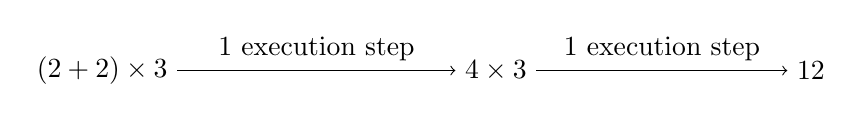
\begin{tikzpicture}[->]

\node (v1) at (-7,0) {$ (2+2) \times 3$};
\node (v2) at (-2,0) {$ 4 \times 3$};
\node (v3) at (2,0) {$ 12 $};
\draw  (v1) -- (v2) node[midway,above] {1 execution step};
\draw  (v2) -- (v3) node[midway,above] {1 execution step};
%\draw (-8.5,-1.5) -- (2.5,-1.5) node[above] {$t$};
\end{tikzpicture}
\par\end{center}

\textbf{Operational semantics }= description of how programs execute.

\end{frame}
%
\begin{frame}{What is a programming language?}

\framesubtitle{A graph whose vertices are programs.}

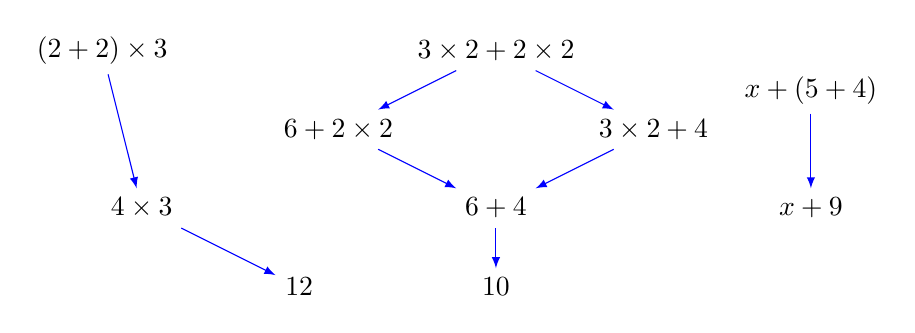
\begin{tikzpicture}[->,draw=blue,>=latex,every edge/.append style = { text=blue}]
%\tikzset{>=latex}

\node (v1) at (-6,11) {$(2+2)\times 3$};
\node (v2) at (-5.5,9) {$4 \times 3$};
  
\node (Omega2) at (-1,11) {$3\times 2 + 2 \times 2$};
\draw  (v1) edge node[sloped, above] {} (v2);
\node (v3) at (-3.5,8) {$12$};
\draw  (v2) edge node[sloped, above] {}(v3);
\node (v7) at (-3,10) {$6+2\times 2$};
\node (v4) at (1,10) {$3\times 2+4$};
\node (v5) at (-1,9) {$6+4$};
\node (v6) at (-1,8) {$10$};
\draw  (Omega2) edge (v4);
\draw  (v4) edge (v5);
\draw  (v5) edge (v6);
\draw  (Omega2) edge (v7);
\draw  (v7) edge (v5);
\node (v8) at (3,10.5) {$x+(5+4)$};
\node (v9) at (3,9) {$x+9$};
\draw  (v8) edge (v9);
\end{tikzpicture}
\vspace{-1.5em} 
\begin{block}{Variables = placeholders for expressions}
\begin{itemize}
\item Substitution: $(x+(5+4))[x:=12]=12+(5+4)$
\item Reductions are stable under substitution
\[
\frac{{\color{red}x}+(5+4)\to\ensuremath{{\color{red}x}+9}}{{\color{red}12}+(5+4)\to{\color{red}12}+9}\,\cdot
\]
\end{itemize}
\end{block}
$\leadsto$ \alert{Reduction monads!}
\end{frame}
%
\begin{frame}{A difficulty}
\begin{alertblock}{Bound variables and $\alpha$-equivalence}

\textbf{$\alpha$-equivalence}:\vspace{-0.5em}
\[
x\mapsto2\times x\quad\text{ should be identified with }\quad y\mapsto2\times y
\]

\begin{center}
``$x$ is bound by $\mapsto$ in $x\mapsto2\times x$''
\par\end{center}

\end{alertblock}
\end{frame}
%
\begin{frame}{Specifying programming languages: \textbf{initial semantics}}
\begin{itemize}
\item Constructing syntax and reductions may be complex (cf.~differential
$\lambda$-calculus).
\item Often easier to describe the \alert{models}.
\end{itemize}
\begin{center}
Model $\approx$ graph with interpretation of the operations and reductions
\par\end{center}
\begin{exampleblock}{a model of arithmetic expressions: $\mathbb{{Z}}$ (or rather $\mathbb{Z}[x,y,\dots]$)}
\begin{itemize}
\item Syntactic ``$+$`` $\qquad\leadsto\qquad$actual ``$+$''�,
\item Syntactic ``$\times$`` $\qquad\leadsto\qquad$actual ``$\times$''�,
...
\end{itemize}
\end{exampleblock}
\begin{itemize}
\item Programming language $=$ \alert{initial} model.
\item Initiality $\Rightarrow$ \alert{recursion principle}.
\end{itemize}
\begin{block}{Notion of signature}
\begin{itemize}
\item Specifies models.
\item \alert{Effective} iff the initial model exists.
\end{itemize}
\end{block}
\end{frame}
%
\begin{frame}{State of the art: syntax}

Two main notions of syntax:
\begin{itemize}
\item \alert{Substitution monoids} ($\approx$ finitary monads) {[}Fiore-Plotkin-Turi,
1999{]}.
\item \alert{Nominal sets} {[}Gabbay-Pitts, 1999{]}.
\end{itemize}
\vspace{1em}

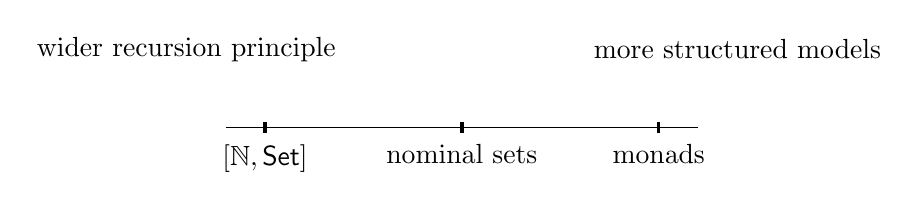
\begin{tikzpicture}
\draw[very thick] (-2.5,2pt)--(-2.5,-2pt) node [below] {$[\mathbb{N},\mathsf{Set}]$};
\draw[very thick] (0,2pt)--(0,-2pt) node [below] {nominal sets};
\draw[very thick] (2.5,2pt)--(2.5,-2pt) node [below] {monads};
\draw (-3,0) -- (3,0);
%\draw[->] (-3,1) edge node[above] {more structured models} (3,1) ;
%\draw[<-] (-3,-1) edge node[below] {wider recursion principle} (3,-1) ;
\node at (3.5,1) {more structured models};
\node at (-3.5,1) {wider recursion principle};
\end{tikzpicture}

\begin{block}{}
This thesis: monads
\end{block}
\end{frame}
%
\begin{frame}{State of the art: specifying syntax}

Main notions of signature for monads:
\begin{itemize}
\item \alert{Pointed strong endofunctors} {[}Fiore-Plotkin-Turi, 1999{]}.
\item \alert{Equational systems} {[}Fiore-Hur, 2010{]}.
\item \alert{Modules} {[}Hirschowitz-Maggesi, 2007{]}.
\end{itemize}
\begin{block}{}
This thesis: modules
\end{block}
\end{frame}
%
\begin{frame}{State of the art: semantics}

Semantic notions of programming language:
\begin{itemize}
\item \alert{Distributive laws} {[}Plotkin-Turi, 1997{]}.
\item \alert{double categories} {[}Meseguer, the Montanari school{]}.
\end{itemize}
Do not cover \alert{higher-order} languages.
\begin{itemize}
\item \alert{2-categories} {[}Power, Seely,...{]}.
\item \alert{relative monads} {[}Ahrens, 2016{]}.
\end{itemize}
Only covers \alert{congruent} semantics.
\end{frame}
%
\begin{frame}{Contributions}
\begin{enumerate}
\item Mathematical definition of programming languages as \textbf{reduction
monads.}
\item Specification of \textbf{syntactic equations}, based on modules over
monads.
\item Specification of \textbf{semantics}.
\end{enumerate}
Systematic use of monads and modules for taking care of substitution.
\begin{block}{Articles}
\begin{itemize}
\item CSL 2018 about 2.
\item FSCD 2019 about 2. = variant of Fiore's approach.
\item POPL 2020 about 1. and 3.
\end{itemize}
\end{block}
All in collaboration with Benedikt Ahrens, Andr� Hirschowitz and Marco
Maggesi.

\textbf{}

\begin{center}
\par\end{center}

\end{frame}

\begin{frame}{Outline}

\tableofcontents{}

\end{frame}

\section{Reduction monads}

\begin{frame}{Ingredients}

\begin{itemize}
\item Programming languages (PLs) as graphs
\begin{itemize}
\item (\textbf{Syntax}) vertices = terms 
\item (\textbf{Semantics}) arrows = reductions between terms
\end{itemize}
\item Simultaneous substitution: variables $\mapsto$ terms
\begin{itemize}
\item monads and modules over them
\end{itemize}
\end{itemize}
\begin{example}
$\lambda$-calculus with $\beta$-reduction:
\begin{itemize}
\item \textbf{Syntax: $\qquad\qquad S,T\quad::=x\mathrel{|}S\,T\mathrel{|}\lambda x.S$}
\item Modulo \textbf{$\alpha$-equivalence}, e.g. 
\[
\lambda x.x=\lambda y.y
\]
\item \textbf{Reductions: }$\qquad\redr{\beta}{(\lambda x.t)\,u}{t[x:=u]}\qquad+\quad\text{congruences}$
\end{itemize}
\end{example}

\end{frame}
%

\subsection{Graphs}
\begin{frame}{PLs as graphs}

\framesubtitle{Example: $\lambda$-calculus with $\beta$-reduction}

\begin{tikzpicture}[->,draw=blue,>=latex,every edge/.append style = { text=blue}]
%\tikzset{>=latex}

\node (v1) at (-6,6.5) {$(\lambda x.x\ y)\ t$};
\node (v2) at (-3,5) {$t\ y$};
\node (Omega) at (-3.5,7.5) {$\Omega$};

\node (Omega2) at (1.5,7.5) {$\Omega\ \Omega$};
\draw  (Omega) edge[loop, looseness=20] node[sloped, above] {$\beta$}(Omega);
\draw  (v1) edge node[sloped, above] {$\beta$}(v2);
\draw  (Omega2) edge[loop, looseness=20] node[sloped, above] {$\beta\ \Omega$}(Omega2);
\draw  (Omega2) edge[loop below, looseness=40] node[sloped, below] {$\Omega\ \beta$}(Omega2);
\end{tikzpicture}


\vspace{-1em}
\begin{columns}
%

\column{\dimexpr\paperwidth-35pt}
\begin{itemize}
\item (\textbf{Syntax}) vertices = terms e.g. $\Omega=(\lambda x.\ x\,x)\,(\lambda x.\ x\,x)$
\item (\textbf{Semantics}) arrows = reductions
\end{itemize}
\end{columns}

\end{frame}
%
\begin{frame}{Graphs}

\framesubtitle{Definition}

Graph = a quadruple $(A,V,\sigma,\tau)$ where 
\begin{align*}
A & =\{\text{arrows}\} & \sigma & =\text{source of an arrow}\\
V & =\{\text{vertices\}} & \tau & =\text{target of an arrow}
\end{align*}
\[
\xymatrix{A\ar@<+.5ex>[r]^{\sigma}\ar@<-0.5ex>[r]_{\tau} & V}
\]

\[
\begin{array}{rcl}
\sigma: & {\color{blue}A} & \to V\\
 & {\color{blue}t\xrightarrow{r}u} & \mapsto t
\end{array}\qquad\begin{array}{rcl}
\tau: & {\color{blue}A} & \to V\\
 & {\color{blue}t\xrightarrow{r}u} & \mapsto u
\end{array}
\]

\[
\sigma(r)\xrightarrow{r}\tau(r)
\]

\end{frame}


\subsection{Substitution}

\begin{frame}{Simultaneous substitution}

\framesubtitle{Syntax comes with substitution}

\framesubtitle{}
\begin{columns}
%

\column{\dimexpr\paperwidth-20pt}

terms (e.g. $\lambda$-terms) = trees with free variables as (distinguished)
leaves.

\end{columns}

\vspace{1em}

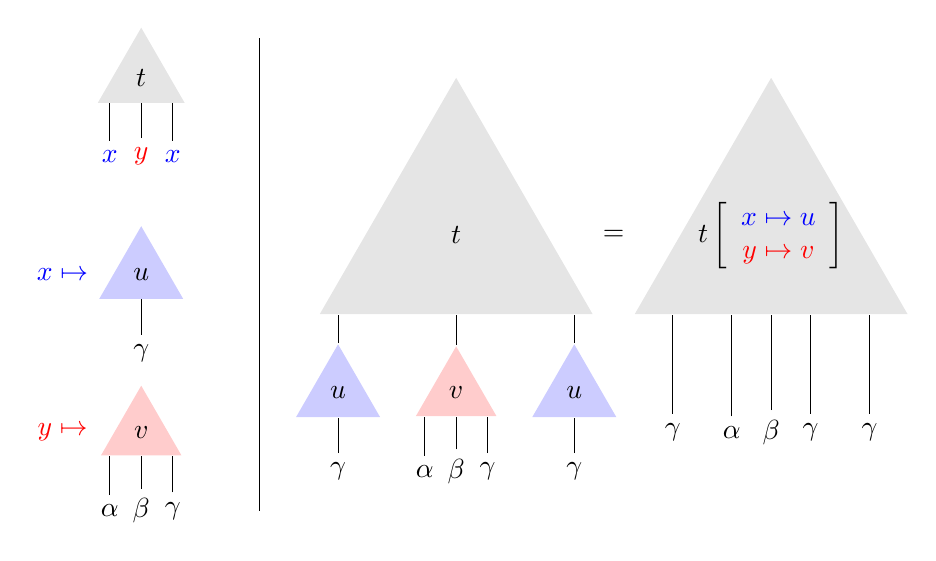
\begin{tikzpicture}[  triangle/.style = 
{fill=blue!20, regular polygon, regular polygon sides=3}]



%
\node[triangle, fill=gray!20] (v1) at (-6.5,5) {$t$};
\node (x1) at (-6.9,4) {$\textcolor{blue}{x}$};
\node (xn) at (-6.1,4) {$\textcolor{blue}{x}$}; 
\node (xi) at (-6.5,4) {$\textcolor{red}{y}$}; 
\draw  (x1.north) edge (x1.north|-v1.south);
\draw  (xn.north) edge (xn.north|-v1.south);
\draw  (xi.north) edge (xi.north|-v1.south);

\node[triangle, fill=blue!20] (u) at (-6.5,2.5) {$u$};
% \node (y1) at (0.1,3.5) {$\alpha$};
% \node (yn) at (0.9,3.5) {$\gamma$}; 
\node (yi) at (-6.5,1.5) {$\gamma$}; 
%\draw  (y1.north) edge (y1.north|-u.south);
%\draw  (yn.north) edge (yn.north|-u.south);
\draw  (yi.north) edge (yi.north|-u.south);

\node[triangle, fill=red!20] (v) at (-6.5,0.5) {$v$};
\node (y11) at (-6.9,-0.5) {$\alpha$};
\node (y1i) at (-6.5,-0.5) {$\beta$}; 
\node (y1n) at (-6.1,-0.5) {$\gamma$}; 
%\node (y1i) at (3.5,0) {$\dots$}; 
\draw  (y11.north) edge (y11.north|-v.south);
\draw  (y1n.north) edge (y1n.north|-v.south);
\draw  (y1i.north) edge (y1i.north|-v.south);

\node[triangle, fill=blue!20] (u2) at (-4,1) {$u$};
%\node (y1) at (2.1,1.5) {$\alpha$};
%\node (yn) at (2.9,1.5) {$\gamma$}; 
\node (yi) at (-4,0) {$\gamma$}; 
%\draw  (y1.north) edge (y1.north|-u2.south);
%\draw  (yn.north) edge (yn.north|-u2.south);
\draw  (yi.north) edge (yi.north|-u2.south);
%

\node[triangle, fill=red!20] (v) at (-2.5,1) {$v$};
\node (y11) at (-2.9,0) {$\alpha$};
\node (y1n) at (-2.1,0) {$\gamma$}; 
\node (y1i) at (-2.5,0) {$\beta$}; 
%\node (y1i) at (3.5,0) {$\dots$}; 
\draw  (y11.north) edge (y11.north|-v.south);
\draw  (y1n.north) edge (y1n.north|-v.south);
\draw  (y1i.north) edge (y1i.north|-v.south);

\node[triangle, fill=blue!20] (u1) at (-1,1) {$u$};
%\node (y1) at (5.1,1.5) {$\alpha$};
%\node (yn) at (5.9,1.5) {$\gamma$}; 
\node (yi) at (-1,0) {$\gamma$}; 
%\draw  (y1.north) edge (y1.north|-u1.south);
%\draw  (yn.north) edge (yn.north|-u1.south);
\draw  (yi.north) edge (yi.north|-u1.south);

\node at (-7.5,2.5) {$\textcolor{blue}{x\mapsto}$};
\node at (-7.5,0.5) {$\textcolor{red}{y\mapsto}$};

%
\node[triangle, fill=gray!20, minimum size=4cm] (v1) at (-2.5,3) {$t$};
%
 
\draw  (u1.north) edge (u1.north|-v1.south);
\draw  (u2.north) edge (u2.north|-v1.south);
\draw  (v.north) edge (v.north|-v1.south);

% \node[triangle, fill=gray!20] (v1) at (0,8) 
% {$t\left[ \begin{array}{c} \textcolor{blue}{x \mapsto u} \\ 
% \textcolor{red}{y \mapsto  v}\end{array}\right]  $};

\node[triangle, fill=gray!20, 
minimum size=4cm,
label=center:{$t\left[ \begin{array}{c} \textcolor{blue}{x \mapsto u} \\ 
\textcolor{red}{y \mapsto  v}\end{array}\right]  $}] (v1) at (1.5,3) {};

\node (v2) at (0.25,0.5) {$\gamma$};
\draw  (v2.north) edge (v2.north|-v1.south);

\node (v2) at (1,0.5) {$\alpha$};
\draw  (v2.north) edge (v2.north|-v1.south);

\node (v2) at (1.5,0.5) {$\beta$};
\draw  (v2.north) edge (v2.north|-v1.south);

\node (v2) at (2,0.5) {$\gamma$};
\draw  (v2.north) edge (v2.north|-v1.south);

\node (v2) at (2.75,0.5) {$\gamma$};
\draw  (v2.north) edge (v2.north|-v1.south);


% \node (v2) at (2,5) {$\gamma$};
% \draw  (v2.north) edge (v2.north|-v1.south);
% \node (v2) at (2.5,5) {$\gamma$};
% \draw  (v2.north) edge (v2.north|-v1.south);

\node at (-0.5,3) {$=$};
\draw (-5,5.5) -- (-5,-0.5);
\end{tikzpicture}

\end{frame}
%
\begin{frame}{Simultaneous substitution made formal}

\framesubtitle{}
\begin{columns}
%

\column{\dimexpr\paperwidth-20pt}
\begin{block}{Free variables indexing}
\[
X\mapsto\{\text{terms taking free variables in \ensuremath{X}}\}
\]

\vspace{-0.5em}
\begin{exampleblock}{Example: $\lambda$-calculus}

\vspace{-1em}

\[
L(\{x,y\})=\left\{
\begin{aligned}
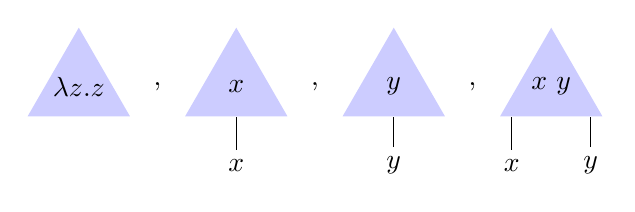
\begin{tikzpicture}
 % \node[triangle, label=center:$\lambda z.z$, minimum size=1.5cm] at (-10.5,4.5) {};
%  \node[anchor=west] at (-9.5,4.5) {$\in L(\emptyset)=\{ \text{closed terms} \}$};
\node[triangle, label=center:$\lambda z.z$, minimum size=1.5cm] at (-16.5,3) {};
%/*
 \node[triangle, label=center:$x$, minimum size=1.5cm] (u) at (-14.5,3) {};
\node (yi) at (-14.5,2) {$x$}; 
\draw  (yi.north) edge (yi.north|-u.south);
\node[triangle, label=center:$y$, minimum size=1.5cm] (u) at (-12.5,3) {};
\node (yi) at (-12.5,2) {$y$}; 
\draw  (yi.north) edge (yi.north|-u.south);
%*/
\node[triangle, label=center:$x\ y$, minimum size=1.5cm] (u) at (-10.5,3) {};
\node (yi) at (-11,2) {$x$}; 
\draw  (yi.north) edge (yi.north|-u.south);
\node (yi) at (-10,2) {$y$}; 
\draw  (yi.north) edge (yi.north|-u.south); 
\node at (-15.5,3) {,};
\node at (-13.5,3) {,};
\node at (-11.5,3) {,};
%\node[anchor=west] at (-9.5,3) {$\in L(\{x,y\})$};
%\node[anchor=east] at (-18.5,3) {$\ L(\{x,y\}) = $};
\end{tikzpicture}
\end{aligned}
,
\dots
\right\}
\]
\end{exampleblock}
\end{block}
%
\begin{block}{Simultaneous substitution}
\[
\forall f:X\rightarrow L(Y),\qquad\boxed{\begin{array}{rl}
L(X) & \rightarrow L(Y)\\
t & \mapsto t[x\mapsto f(x)]\quad\text{(or \ensuremath{t[f]})}
\end{array}}
\]

\end{block}
\end{columns}

\end{frame}
\global\long\def\fauxtext{of}
%
\begin{frame}{Monads model simultaneous substitution}

\framesubtitle{$\lambda$-calculus as a monad $(L,\_[\_],\eta)$}

\begin{enumerate}
\item Simultaneous substitution $(L,\_[\_])$
\item Variables are terms\vspace{-1em}
\[
\begin{array}{cccc}
\eta_{X}: & X & \rightarrow & L(X)\\
 & x & \mapsto & \begin{aligned}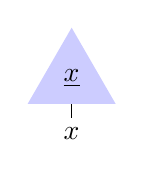
\begin{tikzpicture}\node[triangle](a)at(0,0){\underline{\ensuremath{x}}};\node(b)at(0,-0.7){\ensuremath{x}};\draw(b.north)edge(b.north|-a.south);\end{tikzpicture}\end{aligned}
\end{array}
\]
 
\item Substitution laws:
\[
\underline{x}[f]=f(x)\qquad\qquad t[x\mapsto\underline{x}]=t
\]

+ associativity:
\[
t[f][g]=t\left[x\mapsto f(x)[g]\right]
\]

\end{enumerate}
\end{frame}
%
\begin{frame}{Substitution for semantics}

\framesubtitle{We saw that syntax is expected to support substitution. This is also
true of semantics.}

\framesubtitle{}
\begin{columns}
%

\column{\dimexpr\paperwidth-20pt}

Our notion of PL:
\begin{itemize}
\item \textbf{Syntax}: a monad $(L,\_[\_],\eta)$
\item \textbf{Semantics}:
\begin{itemize}
\item graphs $\xymatrix{R(X)\ar@<+.5ex>[r]^{\sigma_{X}}\ar@<-0.5ex>[r]_{\tau_{X}} & L(X)}
$ for each $X$
\[
R(X)=\begin{array}{c}
\text{total set of reductions between}\\
\text{terms taking free variables in \ensuremath{X}}
\end{array}
\]
\item substitution of reduction: variables \textbf{$\mapsto$ $L$-terms}.
\end{itemize}
\[
\dfrac{\redr rtu}{\redr{r\monsubst f}{t\monsubst f}{u\monsubst f}}
\]

\end{itemize}
\end{columns}

\end{frame}
%
\begin{frame}{Substitution for semantics made formal}

\framesubtitle{}

\begin{columns}
%

\column{\dimexpr\paperwidth-50pt}
\begin{block}{$R$ as a \textbf{module} over $L$}
$R$ supports $L$-monadic substitution:\vspace{-1em}
\[
\forall f:X\rightarrow\boldsymbol{L}(Y),\qquad\boxed{\begin{array}{rl}
R(X) & \rightarrow R(Y)\\
r & \mapsto r[x\mapsto f(x)]\quad\text{(or \ensuremath{r[f]})}
\end{array}}
\]

\begin{center}
\vspace{-0.5em}+ substitution laws
\par\end{center}

\end{block}
\textbf{Other examples of $L$-modules}: $L$, $L\times L$, 1, $\dots$

\begin{block}{$\sigma$ and $\tau$ as \textbf{$L$-module morphisms}}

\[
t\xrightarrow{r}{}u\;\overset{}{\leadsto}\; t'\xrightarrow{r[f]}{}{u'}
\quad
\text{with}
\quad
 \left\{\begin{aligned}
        t'&=t[f] \\
        u'&=u[f]
       \end{aligned}
 \right.
\quad
\text{i.e.,}
\quad
 \left\{\begin{aligned}
       {
%\color{blue}
\sigma(r[f])=\sigma(r)[f]} \\
       {
%\color{blue}
\tau(r[f])=\tau(r)[f]} 
       \end{aligned}
 \right.
\]

\textcolor{blue}{} \vspace{0.3em}

Commutation with substitution $\Leftrightarrow$ Module morphisms
$\sigma,\tau:R\rightarrow L$.
\end{block}
\end{columns}

\end{frame}
%
\begin{frame}{Reduction monads}

\framesubtitle{Summary: graphs + substitution.}
\begin{definition}
A \textbf{reduction monad}  $\xymatrix{R\ar@<+.5ex>[r]^{\sigma}\ar@<-0.5ex>[r]_{\tau} & T}
$ consists of
\begin{itemize}
\item $T$ = monad (= module over itself)
\item $R$ = module over $T$
\item $\sigma,\tau:R\rightarrow T$ are $T$-module morphisms.
\end{itemize}
\end{definition}

\begin{example}
$\lambda$-calculus with $\beta$-reduction.
\end{example}

\textbf{How can we specify a reduction monad?}
\begin{enumerate}
\item  signature for the (syntactic) operations for the monad;
\item  reduction rules.
\end{enumerate}

\end{frame}

\section{Syntax}

\begin{frame}{Overview}
\begin{itemize}
\item Syntax = monad $L$
\item Operations = module morphisms $\Sigma(L)\rightarrow L$
\item 1-signatures specify operations
\item 2-signatures specify operations + equations.
\end{itemize}
\end{frame}
%

\subsection{Operations}
\begin{frame}{Operations as module morphisms}

\includegraphics[width=1\textwidth]{images/operations-as-module-morphisms}
\end{frame}
%
\begin{frame}{Examples of modules}

\framesubtitle{We argued that syntactic operations are \textbf{module morphisms}.
Basic examples of modules?}

\textbf{Module over a monad }$T$: supports the $T$-monadic substitution
\begin{exampleblock}{Examples}
\textbf{}
\begin{itemize}
\item $T$ itself
\item $M\times N$ for any modules $M$ and $N$:
\[
\forall(t,u)\in M(X)\times N(X),\quad\qquad X\xrightarrow{f}T(Y),
\]
\[
\boxed{(t,u)[f]=(t[f],u[f])}\in M(Y)\times N(Y)
\]
\item $M'$= \textbf{derivative} of a module $M$:\textrm{\vspace{2em}}
\end{itemize}
\[
M'(X)=M(\tikzmarknode{freshv}{X\amalg\{\diamond\}})
\]
\begin{tikzpicture}[overlay, remember picture]
  \draw[decorate,decoration={brace, amplitude=1.5ex}] 
%    ([yshift=1ex]:#2.north east)  --  (#3.south east-|#2.north east)
    (freshv.north west)  --  (freshv.north east) node[ above=.6em]{$X$ extended with a fresh variable $\diamond$};
%\node[above right= 1cm of freshv] (legfreshv) {fresh variable};
%\draw[->] (legfreshv) to[bend right] (freshv);
\end{tikzpicture}used to model an operation binding a variable (Cf next slide).

\end{exampleblock}
\end{frame}
%
\begin{frame}{Operations as module morphisms}

\framesubtitle{Operations can be combined into a single one.}
\begin{columns}
%

\column{\dimexpr\paperwidth-35pt}

Operations = module morphisms\textbf{ }= maps commuting with substitution:

\end{columns}

\begin{exampleblock}{Example: $\lambda$-calculus}

\[
\begin{array}{rcl}
\app: & L\times L & \rightarrow L\\
\abs: & L' & \rightarrow L\qquad\left\{ \quad\begin{aligned}\abs_{X}:L(X\amalg\{\diamond\}) & \rightarrow L(X)\\
t & \mapsto\lambda\diamond.t
\end{aligned}
\right.
\end{array}
\]

Combine operations into a single one:
\[
\boxed{[\app,\abs]:(L\times L)\amalg L'\rightarrow L}
\]
where (\emph{coproducts} of modules $M$ and $N$)
\[
(M\amalg N)(X)=M(X)\amalg N(X)
\]

\end{exampleblock}
\end{frame}
%
\begin{frame}{1-signatures specify operations}
\begin{definition}
A \textbf{1-signature} $\Sigma$ is a (functorial) assignment

\vspace{-1em}
\[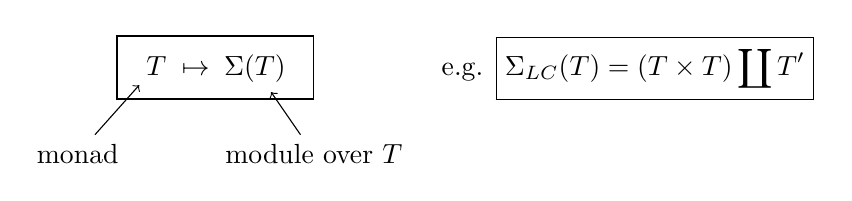
\begin{tikzpicture}[->]
% \node (v2) at (0,0) {$\boxed{T\mapsto \Sigma(T)}$};
\node (v1) at (-0.5,-1) {monad};
\node (v2) at (2.5,-1) {module over $T$};
\node[anchor=base] at (1,0) {$\mapsto$};
\node[anchor=base] (v3) at (1.75,0) {$\Sigma(T)$};
\node[anchor=base] (v4) at (0.5,0) {$T$};
\draw  (v2) edge (v3);
\draw  (v1) edge (v4);
\draw  (0,0.5) rectangle (2.5,-0.3);
\node[anchor=base west] at (4,0) {e.g. $\boxed{\Sigma_{LC}(T)=(T\times T)\coprod T'}$};
\end{tikzpicture}\]
\end{definition}

\begin{definition}
[model of a 1-signature $\Sigma$]A \textbf{model} of $\Sigma$ is
a pair $(T,m)$ denoted by $\Sigma(T)\xrightarrow{m}T$ s.t.
\begin{itemize}
\item $T$ is a monad
\item $\Sigma(T)\xrightarrow{m}T$ is a $T$-module morphism
\end{itemize}
\end{definition}

\begin{exampleblock}{Example: $\lambda$-calculus}
\vspace{-1em}
\[
[\app,\abs]:\Sigma_{LC}(L)\rightarrow L\qquad\text{where }\Sigma_{LC}(L)=(L\times L)\amalg L'
\]
\end{exampleblock}

\end{frame}

\begin{frame}{Syntax}

\framesubtitle{We defined 1-signatures and their models. When is a signature effective?}

(suitable notion of model morphism {[}Hirschowitz-Maggesi 2012{]})
\begin{definition}
The\textbf{ syntax} specified by a 1-signature $\Sigma$ is the initial
object in its category of models.
\end{definition}

\begin{description}
\item [{Question:}] Does the syntax exist for every 1-signature?
\item [{Answer:}] No.
\item [{Counter-example:}] $\Sigma(R)=\tikzmarknode{P}{\mathcal{P}}\circ R$
\end{description}
\vspace{1em}

\begin{center}
\tikzmarknode{dP}{Powerset endofunctor on $Set$.}
\end{center}
\begin{tikzpicture}[remember picture,overlay]
\draw[->] (dP) -- (P);
\end{tikzpicture}

(for cardinality reasons)

\begin{center}
\par\end{center}

%\begin{tikzpicture}[->, overlay,remember picture]
%  \node[below left=of pic cs:P] (yop) {yop};
%  \draw (yop)  --  ($ (pic cs:P) $);
%  \draw ($ (pic cs:yop) $)  --  ($ (pic cs:P) $);
%\end{tikzpicture}

\end{frame}

\begin{frame}{Initial semantics for algebraic 1-signatures}

\framesubtitle{We gave examples of effective 1-signatures. They were all \textbf{algebraic}.}

\begin{columns}
    \column{\dimexpr\paperwidth-50pt}
\begin{definition}
\textbf{Algebraic 1-signatures }= 1-signatures built out of derivatives,
finite products, disjoint unions, and the 1-signature $\Theta:T\mapsto T$.
\end{definition}

Algebraic 1-signatures $\simeq$ binding signatures {[}Fiore-Plotkin-Turi
1999{]}

$\Rightarrow$ specification of $n$-ary operations, possibly binding
variables.
\begin{theorem}
[Fiore-Plotkin-Turi 1999]Syntax exists for any algebraic 1-signature.
\end{theorem}

\begin{example}
$\lambda$-calculus
\end{example}

\textbf{Question}: Specify syntactic operations subject to some equations?

\begin{center}
(\emph{commutative} \emph{associative} binary operation $+$ of diff.
$\lambda$-calculus)
\par\end{center}

\end{columns}
\end{frame}
%
\begin{frame}{Quotient of algebraic signatures}

We saw that algebraic signatures are effective. Can we specify effectively
operations subject to equations?
\begin{theorem}
[CSL 2018]\tikzmark{onethm}Syntax exists for any ``quotient''
of algebraic 1-signatures.
\end{theorem}

\begin{example}
a \emph{commutative} binary operation $+$: 
\[
\forall a,b,\quad a+b=b+a
\]
\end{example}

\end{frame}
{ % all template changes are local to this group.
    \setbeamertemplate{navigation symbols}{}
    \begin{frame}[plain]
        \begin{tikzpicture}[remember picture,overlay]
            \node[at=(current page.center)] {

 \includegraphics[keepaspectratio, width=\paperwidth]{images/thinkingguepard} 
% \includegraphics{images/thinkingguepard}

                
            };
        \end{tikzpicture}
     \end{frame}
}

\subsection{Equations}

\begin{frame}{Example: a commutative binary operation}
\begin{block}{Specification of a binary operation}
\begin{center}
\begin{tabular}{c|c}
1-signature & $T\mapsto T\times T$\tabularnewline
\hline 
model & $
%\begin{pmatrix}
\begin{array}{c}
\xymatrix@R=1em{T \times T \ar[d]^+ \\ T}
\end{array}
%\end{pmatrix}
$\tabularnewline
\end{tabular}
\par\end{center}
\end{block}
\begin{description}
\item [{Question}] What is an appropriate notion of model for a \textbf{commutative
}binary operation?
\end{description}
\begin{itemize}
\item a monad $T$\tikzmark{monad}
\item with a binary operation\tikzmark{binop} \VerticalBrace{monad}{binop}{a model $T\times T\xrightarrow{+}{}T$ of $\Theta\times\Theta$}
\item s.t.
\end{itemize}
\[
\xymatrix@R=0.25em{T\times T 
\ar@/^+1.5em/[rr]^+
\ar@/^-0.5em/[rd]_{\text{swap}}
 &  & T\\
 & T\times T
\ar@/^-0.5em/[ru]_+
}
\qquad
\text{where}\quad\text{swap}(t,u) = (u,t)
\]

\end{frame}

\begin{frame}{Equations}

$\Sigma=$ 1-signature (e.g. binary operation $\Sigma(T)=T\times T)$
\begin{definition}
A \textbf{$\Sigma$-equation} $\xymatrix{A\ar@<+.5ex>^{u}[r]\ar@<-.5ex>_{v}[r] & B}
$ is a (functorial) assignment

\vspace{-1em}\[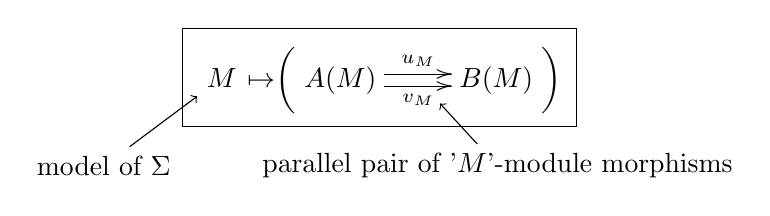
\begin{tikzpicture}[->]
% \node (v2) at (0,0) {$\boxed{T\mapsto \Sigma(T)}$};
\node (v1) at (-1,-1) {model of $\Sigma$};
\node (v2) at (4,-1) {parallel pair of '$M$'-module morphisms} ;
\node[anchor=base] at (1,0) {$\mapsto$};
\node[anchor=base] (v3) at (3,0) {$\left(
	\xymatrix{A(M)\ar@<+.5ex>^{u_M}[r]\ar@<-.5ex>_{v_M}[r] & B(M)}
	\right)$};
\node[anchor=base] (v4) at (0.5,0) {$M$};
\draw[shorten >= -10pt]  (v2) edge (v3);
\draw  (v1) edge (v4);
\draw  (0,0.75) rectangle (5,-0.5);
% \node[anchor=base west] at (5,0) {e.g. $\boxed{
% %T\times T\xrightarrow{+}{} T
% \begin{array}{c}
% \xymatrix@R=1em{T\times T\ar[d]^+ \\ T}
% \end{array}
% \mapsto
% \xymatrix@R=0.25em@C=1em{T\times T 
% \ar@/^+1.5em/[rr]^+
% \ar@/^-0.5em/[rd]_-{\text{swap}}
%  &  & T\\
%  & T\times T
% \ar@/^-0.5em/[ru]_-+
% }	 
% 	}$};
\end{tikzpicture}
\]

\end{definition}

\begin{example}
[Binary commutative operation]
\vspace{-1em}
\[
\Sigma(T)=T\times T
\qquad
\left|
\quad 
%\boxed{
{
%T\times T\xrightarrow{+}{} T
\begin{array}{c}
\xymatrix{T\times T\ar[d]^+ \\ T}
\end{array}
\mapsto
\xymatrix@R=0.25em@C=1em{T\times T
\ar@/^+1.5em/[rr]^+
\ar@/^-0.5em/[rd]_-{\text{swap}}
 &  & T\\
 & T\times T
\ar@/^-0.5em/[ru]_-+
}       
        }
\right.
\]

\end{example}

\end{frame}
%
\begin{frame}{2-signatures and their models}

\framesubtitle{We defined equations. A set of equations yields a 2-signature.}
\begin{definition}
A\textbf{ 2-signature} is a pair $(\Sigma,E$) where
\begin{itemize}
\item $\Sigma$ is a 1-signature for monads
\item $E$ is a set of $\Sigma$-equations
\end{itemize}
\end{definition}

\begin{definition}
A\textbf{ model} of a 2-signature $(\Sigma,E$) consists of:
\begin{itemize}
\item a model $ M = \begin{pmatrix}\xymatrix@R=1em{\Sigma(T)\ar[d]\\T}\end{pmatrix}$
of $\Sigma$ s.t.
\[
\forall\xymatrix{A\ar@<+.5ex>^{u}[r]\ar@<-.5ex>_{v}[r] & B}
\in E,\quad\boxed{u_{M}=v_{M}}:A(M)\rightarrow B(M)
\]
\end{itemize}
\end{definition}

morphism of models = morphisms as models of $\Sigma$.

\end{frame}
%
\begin{frame}{Initial semantics for algebraic 2-signatures}

\framesubtitle{We defined 2-signatures and their models. When is a 2-signature effective?}

\begin{theorem}
[FSCD 2019]\tikzmark{twothm}Any \textbf{algebraic} 2-signature has
an initial model.
\end{theorem}

\begin{definition}
A 2-signature $(\Sigma,E)$ is \textbf{algebraic} if:
\begin{itemize}
\item $\Sigma$ is algebraic
\item $E$ consists of \textbf{elementary $\Sigma$}-equations
\end{itemize}
\end{definition}

\begin{exampleblock}{Main instances of elementary $\Sigma$-equations}

\vspace{-1em}
\[
A\rightrightarrows B \text{ s.t.}\qquad
A\begin{pmatrix}
\small
\xymatrix@R=0.8em{\Sigma(T)\ar[d]\\
T
}
\end{pmatrix}=\Phi(T)\qquad 
%
B\begin{pmatrix}
\small
\xymatrix@R=0.8em{\Sigma(T)\ar[d]\\
T
}
\end{pmatrix}
=T
\]

\vspace{-0.5em}for some \emph{algebraic} 1-signature $\Phi$.
\begin{center}
\vspace{-0.5em}(e.g. $\Phi(T)=T\times T$ for commutativity)
\par\end{center}

\end{exampleblock}
\end{frame}

\begin{frame}{Example: algebraic 2-signature for differential $\lambda$-calculus}

\framesubtitle{Lionel Vaux's version}

\vspace{-1em}
\[
\begin{array}{ccccccccc}
L^{d}:\quad s,t & ::= & x\mathop{|}s\,t\mathop{|}\lambda x.s & | & Ds\cdot t & | & 0 & | & s+t\\
\Sigma_{LC^{d}}(T) & = & \Sigma_{LC}(T) & \amalg & T\times T & \amalg & 1 & \amalg & T\times T
\end{array}
\]
\vspace{-1em}
\begin{block}{Equations}
\begin{itemize}
\item \emph{associativity }and \emph{commutativity} of $+,$ neutrality
of $0$ for $+$
\item bilinearity of $D\_\cdot\_$ with respect to $+$, left linearity
of application, linearity of abstraction
\[
\lambda x.(s+t)=\lambda x.s+\lambda x.t\qquad\lambda x.0=0
\]
 
\end{itemize}
\end{block}
%

\end{frame}

\section{Semantics}

\begin{frame}{Specifying reduction monads}

$\lambda$-calculus with (small-step) $\beta$-reduction as a reduction
monad: 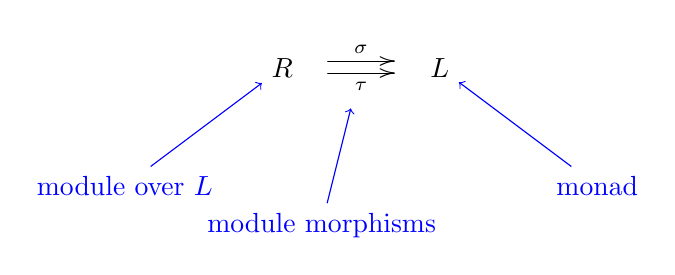
\begin{tikzpicture}[->]

\node (v2) at (-0.5,0) {$ \xymatrix{\ar@<+.5ex>[r]^{\sigma}\ar@<-0.5ex>[r]_{\tau} & }  $};
  
\node[blue] (v4) at (2.5,-1.5) {monad};
\node[blue] (v1) at (-3.5,-1.5) {module over $L$};
\node (v3) at (-1.5,0) {$R$};
\node  (v5) at (0.5,0) {$L$};
\draw[blue]  (v1) edge (v3);
\draw[blue]  (v4) edge (v5);
\node[blue] (v6) at (-1,-2) {module morphisms};
\draw[blue]  (v6) edge (v2);
\end{tikzpicture}

\begin{itemize}
\item vertices = $L$ = initial model of the signature of $\lambda$-calculus.
\item arrows = $R,\sigma,\tau$ = ? 
\begin{itemize}
\item specified through \emph{reduction rules }(to be made formal):
\[
(\lambda x.t)\,u\rightarrow t[x:=u]\qquad\frac{t\rightarrow t'}{t\,u\rightarrow t'\,u}\qquad\dots
\]
\end{itemize}
\end{itemize}
\end{frame}


\subsection{Reduction rules}
\begin{frame}{Analysis of a reduction rule}

\framesubtitle{Example: binary congruence for application.}
\begin{columns}
%

\column{\dimexpr\paperwidth-20pt}

\vspace{-0.5em}

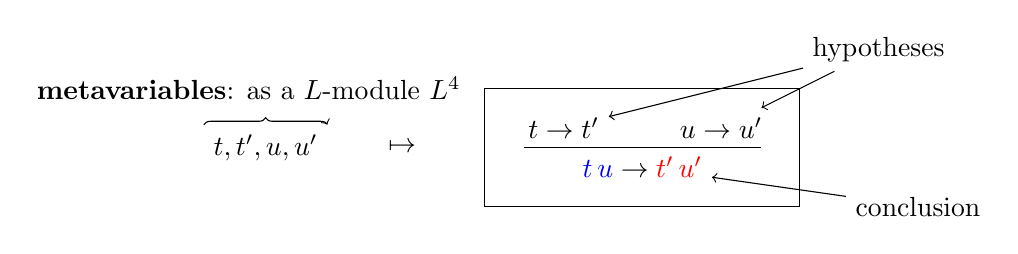
\begin{tikzpicture}[->]


\draw[-] (-4,2.75) -- (-1,2.75);

\node (v8) at (-3.5,3) {$t\rightarrow t'$};
\node (v9) at (-1.5,3) {$u\rightarrow u'$}; 
\node (v11) at (-2.5,2.5) {${\color{blue}t\,u}\rightarrow{\color{red}t'\,u'}$};
\draw  (-4.5,3.5) rectangle (-0.5,2);
\node (v7) at (0.5,4) {hypotheses};
\node (v10) at (1,2) {conclusion};
\draw  (v7) edge (v8);
\draw  (v7) edge (v9);
\draw  (v10) edge (v11);
% \node[anchor=west] at (1,3) {metavariables: $t,t',u,u'$};
% \node[anchor=west] at (1,2.5) {$\Rightarrow$ as a $L$-module: $L^4$};
\node[anchor=east] (mv) at (-6.5,2.75) {$t,t',u,u'$};
\draw[decorate, decoration = brace] (mv.north west) -- (mv.north east);
% \node[midway, above] {metavariables};
\node[anchor=east] at (-5.25,2.75) {$\mapsto$};
\node at (-7.5,3.5) {\textbf{metavariables}: as a $L$-module $L^4$};
\end{tikzpicture}
\vspace{-1em}

Hypothesis/conclusion = pair of \emph{$\lambda$-}terms using metavariables
\begin{itemize}
\item as parallel module morphisms $L^{4}\rightrightarrows L$
\item \textbf{Generalization}: $L\leadsto$ any model $\Sigma_{LC}(T)\rightarrow T$
of $\Sigma_{LC}$:
\begin{center}
(application denoted by $\app:T\times T\rightarrow T$)
\begin{align*}
\text{e.g.,}\quad{\color{blue}t\,u}\rightarrow{\color{red}t'\,u'}:\qquad\qquad T^{4} & \rightarrow T\\
(t,t',u,u') & \mapsto{\color{blue}\app(t,u)}\\
(t,t',u,u') & \mapsto{\color{red}\app(t',u')}
\end{align*}
\par\end{center}

\end{itemize}
\end{columns}

\end{frame}
%
\begin{frame}{Reduction rules}

\framesubtitle{Definition}
\begin{columns}
%

\column{\dimexpr\paperwidth-20pt}

\vspace{-0.5em}Let $\Sigma$ = signature for monads (e.g. $\Sigma_{LC}$
for congruence for application).

\end{columns}

\begin{columns}
%


\column{\dimexpr\paperwidth-40pt}

\begin{block}{Definition of $\Sigma$-reduction rules}

A \textbf{$\Sigma$-reduction rule }$(\vec{\sigma},\vec{\tau})$ $\qquad\quad\boxed{\dfrac{\sigma_{1}\rightarrow\tau_{1}\quad\dots\quad\sigma_{n}\rightarrow\tau_{n}}{\sigma_{0}\rightarrow\tau_{0}}}$

\vspace{1em}

assigns (functorially) to each model $\Sigma(T)\rightarrow T$:

\hfill\tikzmark{right}
\begin{itemize}
\item $V(T)$ = $T$-module of metavariables (e.g. $V(T)=T^{4}$) 
\item parallel $T$-module morphisms $\xymatrix{V(T)\ar@<+.5ex>[r]^{\sigma_{i,T}}\ar@<-.5ex>[r]_{\tau_{i,T}} & {{T'}^{\dots}\tikzmark{e}}{}'}
$
\end{itemize}
We write\vspace{-1em}
\[
\sigma_{i},\tau_{i}:V\rightarrow\Theta^{(n_{i})}\qquad n_{i}=\text{number of \ensuremath{\overset{\tikzmark{dd}}{\text{derivatives}}}}
\]
\begin{tikzpicture}[->, overlay,remember picture]
  \draw ($ (pic cs:dd) $)  --  ($ (pic cs:e) $);
\end{tikzpicture}
\vspace{-2em}

\end{block}
\end{columns}

\end{frame}

\subsection{Reduction signatures\protect 
%
}\begin{frame}{Reduction signatures}

Reduction signatures specify reduction monads.
\begin{block}{Definition}

A\textbf{ reduction signature} is a pair $(\Sigma,\text{\ensuremath{\mathfrak{R}}}$)
where
\begin{itemize}
\item $\Sigma$ is a signature for monads (1- or 2-signature)
\item $\mathfrak{R}$ is a family of $\Sigma$-reduction rules
\end{itemize}
\end{block}
\begin{exampleblock}{Example: $\lambda$-calculus with $\beta$-reduction}
\begin{itemize}
\item $\Sigma=\Sigma_{LC}$
\item $\Sigma$-reduction rules:
\begin{itemize}
\item $\beta$-reduction
\item congruences for application and abstraction
\end{itemize}
\end{itemize}
\end{exampleblock}
\end{frame}
%
\begin{frame}{Models}

\framesubtitle{We defined \textbf{reduction signatures}. What are their models?}

A \textbf{model} of a signature $(\Sigma,\mathfrak{R})$ consists
of:
\begin{itemize}
\item a reduction monad $\xymatrix{R\ar@<+.5ex>[r]^{\sigma}\ar@<-.5ex>[r]_{\tau} & T}
$ with a $\Sigma$-model structure on $T$
\item for each reduction rule 
\[
\boxed{\dfrac{\sigma_{1}\rightarrow\tau_{1}\quad\dots\quad\sigma_{n}\rightarrow\tau_{n}}{\sigma_{0}\rightarrow\tau_{0}}{}_{op}}\text{\ensuremath{\quad\xymatrix{V\xyport{{\xyarrow[r][][][][0.5ex]}}{\sigma_{i}}-\xystarboard{{\xyarrow[r][][][][-0.5ex]}}{\tau_{i}}- & \Theta^{(n_{i})}}
}}\quad\text{in \ensuremath{\mathfrak{R}},}
\]

\begin{itemize}
\item \vspace{-0.4em} a mapping, for each $v\in V(T)(X)$,\vspace{-0.5em}
\[
\begin{pmatrix}\redr{r_{1}}{\sigma_{1}(v)}{\tau_{1}(v)}\\
\dots\\
\redr{r_{n}}{\sigma_{n}(v)}{\tau_{n}(v)}
\end{pmatrix}\quad\mapsto\quad\redr{op(r_{1},\dots r_{n})}{\sigma_{0}(v)}{\tau_{0}(v)}
\]
\item compatible with substitution:\vspace{-0.5em}
\[
op(r_{1},\dots r_{n})[f]=op(r_{1}[f],\dots,r_{n}[f])
\]
\end{itemize}
\end{itemize}
\end{frame}
%
\begin{frame}{Initiality}

\framesubtitle{We defined \textbf{models }of a \textbf{reduction signature}. When
is a signature effective?}

(suitable notion of model morphism)
\begin{theorem}
[POPL 2020]$\Sigma$ has an initial model (e.g. $\Sigma$ is algebraic)
$\Rightarrow$ $(\Sigma,\mathfrak{R})$ has an initial model.
\end{theorem}

\begin{exampleblock}{Examples}
\begin{itemize}
\item $\lambda$-calculus with small-step $\beta$-reduction
\item $\lambda$-ex = $\lambda$-calculus with explicit substitutions {[}Kesner
2009{]}.
\end{itemize}
\begin{center}
\emph{\small{}\vspace{-0.5em}A Theory of Explicit Substitutions with
Safe and Full Composition}{\small\par}
\par\end{center}

\end{exampleblock}
\end{frame}
%
\begin{frame}{Reduction signature for $\lambda$-ex}
\begin{block}{Syntax}

$\lambda$-ex: $\lambda$-calculus + explicit substitution $t[x/u]$
s.t. $x$ is bound in $t$:\vspace{-0.5em}
\begin{center}
as a module morphism ${\color{blue}L^{ex}{}'\times L^{ex}}\rightarrow L^{ex}$\vspace{-0.5em}
\[
\boxed{\Sigma_{\lambda\text{-ex}}(T)=\Sigma_{LC}(T)\amalg{\color{blue}(T'\times T)}}
\]
\vspace{-3em}
\par\end{center}

subject to the equation\vspace{-0.5em}
\[
\boxed{t[x/u][y/v]=t[y/v][x/u]}\quad\text{if {\color{green}\ensuremath{y\notin fv(u)}} and {\color{green}\ensuremath{x\notin fv(v)}}}
\]
as a $\Sigma_{L^{ex}}$-equation $L^{ex}{}''\times{\color{green}L^{ex}}\times{\color{green}L^{ex}}\rightrightarrows L^{ex}$.

\end{block}
%
\begin{block}{Semantics}

congruences, $\beta$-reduction \textrm{$(\lambda x.t)\,u\rightarrow t[x/u]$,
$\dots$}
\[
t[x/u][y/v]\rightarrow t[y/v][x/u[y/v]]\quad\text{if {\color{green}\ensuremath{x\notin fv(u)}} and {\color{red}\ensuremath{y\in fv(u)}}}
\]

metavariable module: $L^{ex}{}''\times{\color{green}L^{ex}}\times{\color{red}L_{\diamond}^{ex}}\qquad\quad(L_{\diamond}^{ex}\subset L^{ex}{}')$

\end{block}
\end{frame}

\begin{frame}{Extension of reduction monads}

\framesubtitle{with associated effectivity theorem}
\begin{enumerate}
\item Vertices: syntax/monad $\leadsto$ module of ``configurations''
over the syntax
\begin{exampleblock}{Examples}
\begin{itemize}
\item $\lambda$-calculus with small-step $\beta$-reduction cbv:
\begin{itemize}
\item variables $\mapsto$ \textbf{values }(rather than terms)
\item Thus, monad of \textbf{values} (rather than terms)
\item Still, reductions between \textbf{terms} (rather than values) = ``configurations''
over the monad of values
\end{itemize}
\item $\pi$-calculus
\item differential $\lambda$-calculus (without its signature though)
\end{itemize}
\end{exampleblock}
\item Graph $\leadsto$ Bipartite graph
\begin{example}
$\lambda$-calculus with big-step $\beta$-reduction cbv: term $\rightarrow$
value.
\end{example}

\end{enumerate}
\end{frame}

\section*{Conclusion}
\begin{frame}{Conclusion}
\begin{block}{Summary}
\begin{itemize}
\item PLs as reduction monads
\item Signatures for reduction monads with effectivity theorem
\end{itemize}
\end{block}
%
\begin{block}{Perspectives}
\begin{itemize}
\item Generalize reduction monads and their signatures
\begin{itemize}
\item specify the differential $\lambda$-calculus
\end{itemize}
\item Generalize on the category of sets:
\begin{itemize}
\item specify simply-typed PLs: category of families of sets (indexed by
simple types) 
\item specify Finster-Mimram's monad of weak $\omega$-groupoids: category
of globular sets
\end{itemize}
\end{itemize}
\end{block}

\end{frame}

\appendix

\end{document}
